
\documentclass[11pt,a4paper]{article}

\usepackage[utf8]{inputenc}
\usepackage[T1]{fontenc}
\usepackage[polish]{babel}
\usepackage[margin=2cm]{geometry}
\usepackage{xltabular}
\usepackage{tabularx}
\usepackage{array}
\usepackage{graphicx}

\setlength{\parindent}{0pt}
\renewcommand{\arraystretch}{1.3}
\setlength{\tabcolsep}{5pt}

\newcolumntype{Y}{
>{\raggedright\arraybackslash}X
}

\newcommand{\naglowek}{
\hline
\textbf{Jako...} &
\textbf{Chcę...} &
\textbf{Aby...} \\
\hline
}

\newcommand{\pole}[2]{
\textbf{#1} & #2 \\ \hline
}

\begin{document}

\begin{center}
{\LARGE \textbf{PsychSearch}}
\end{center}

\vspace{0.5cm}

\section*{Aktorzy systemu}

W ramach platformy PsychSearch zdefiniowano
trzy główne role (aktorów) wchodzące
w interakcję z systemem:

\begin{itemize}

\item \textbf{Użytkownik} -
osoba poszukująca wsparcia psychologicznego.
Korzysta z aplikacji w celu znalezienia
odpowiedniego specjalisty, przeglądania
wolnych terminów oraz umawiania się
na konsultacje.

\item \textbf{Psycholog} -
zweryfikowany specjalista świadczący
usługi psychologiczne. Korzysta z systemu,
aby zarządzać swoim profilem zawodowym,
ustalać grafik dostępności oraz przyjmować
lub odrzucać prośby o konsultacje
od użytkowników.

\item \textbf{Administrator} -
osoba odpowiedzialna za nadzór nad całą
platformą. Dba o poprawne funkcjonowanie
systemu, weryfikuje profile specjalistów,
rozwiązuje problemy techniczne i pilnuje
przestrzegania regulaminu.

\end{itemize}

\vspace{0.5cm}

\section*{User Stories}

\begin{xltabular}{\textwidth}{|p{2.5cm}|Y|Y|}

\naglowek
\endfirsthead

\naglowek
\endhead

Użytkownik &
założyć konto w aplikacji PsychSearch &
móc korzystać z funkcjonalności systemu. \\
\hline

Użytkownik &
przeglądać listę dostępnych psychologów &
znaleźć odpowiedniego specjalistę. \\
\hline

Użytkownik &
wyświetlić profil wybranego psychologa &
zapoznać się z jego specjalizacjami. \\
\hline

Użytkownik &
sprawdzać dostępne terminy konsultacji &
wybrać dogodny dla mnie termin. \\
\hline

Użytkownik &
wysłać prośbę o konsultację
do wybranego psychologa &
umówić się na wizytę. \\
\hline

Użytkownik &
sprawdzać status mojej konsultacji &
wiedzieć, czy została zaakceptowana,
odrzucona lub oczekuje na decyzję. \\
\hline

Użytkownik &
otrzymywać powiadomienia o zmianach
statusu konsultacji &
być na bieżąco z decyzją psychologa. \\
\hline

Użytkownik &
anulować wysłaną prośbę
lub zaakceptowaną wizytę &
móc zrezygnować z konsultacji. \\

\noalign{\hrule height 2pt}


Psycholog &
założyć konto w aplikacji PsychSearch &
móc oferować konsultacje użytkownikom. \\
\hline

Psycholog &
dodawać i edytować swoje specjalizacje &
użytkownicy mogli znaleźć mnie
na podstawie swoich potrzeb. \\
\hline

Psycholog &
dodawać, zmieniać i usuwać dostępne
terminy konsultacji &
dostosować harmonogram do mojej
dyspozycyjności. \\
\hline

Psycholog &
otrzymywać prośby o konsultacje
od użytkowników &
móc rozpatrywać nowe zgłoszenia. \\
\hline

Psycholog &
przeglądać otrzymane prośby
o konsultacje &
planować czas i korelować z innymi terminami.\\
\hline

Psycholog &
akceptować otrzymane prośby
o konsultacje &
potwierdzać użytkownikom możliwość
odbycia wizyty w wybranym terminie. \\
\hline

Psycholog &
odrzucać otrzymane prośby
o konsultacje &
informować użytkowników o braku
możliwości odbycia wizyty. \\
\hline

Psycholog &
sprawdzać aktualne statusy konsultacji &
mieć kontrolę nad zaplanowanymi
wizytami. \\

\noalign{\hrule height 2pt}

Administrator &
zarządzać kontami użytkowników
i psychologów &
zapewnić prawidłowe funkcjonowanie
aplikacji. \\
\hline

Administrator &
weryfikować profile psychologów &
zapewnić wiarygodność specjalistów
dostępnych w systemie. \\
\hline

Administrator &
diagnozować i rozwiązywać
problemy techniczne &
zapewnić prawidłowe działanie
aplikacji. \\
\hline

Administrator &
blokować konta użytkowników
i psychologów naruszających regulamin &
zapewnić bezpieczeństwo pozostałym
użytkownikom systemu. \\
\hline

\end{xltabular}


\clearpage

\section*{Diagram przypadków użycia}

\begin{figure}[htbp]
    \centering
    % width=\textwidth dopasowuje szerokość diagramu do szerokości tekstu
    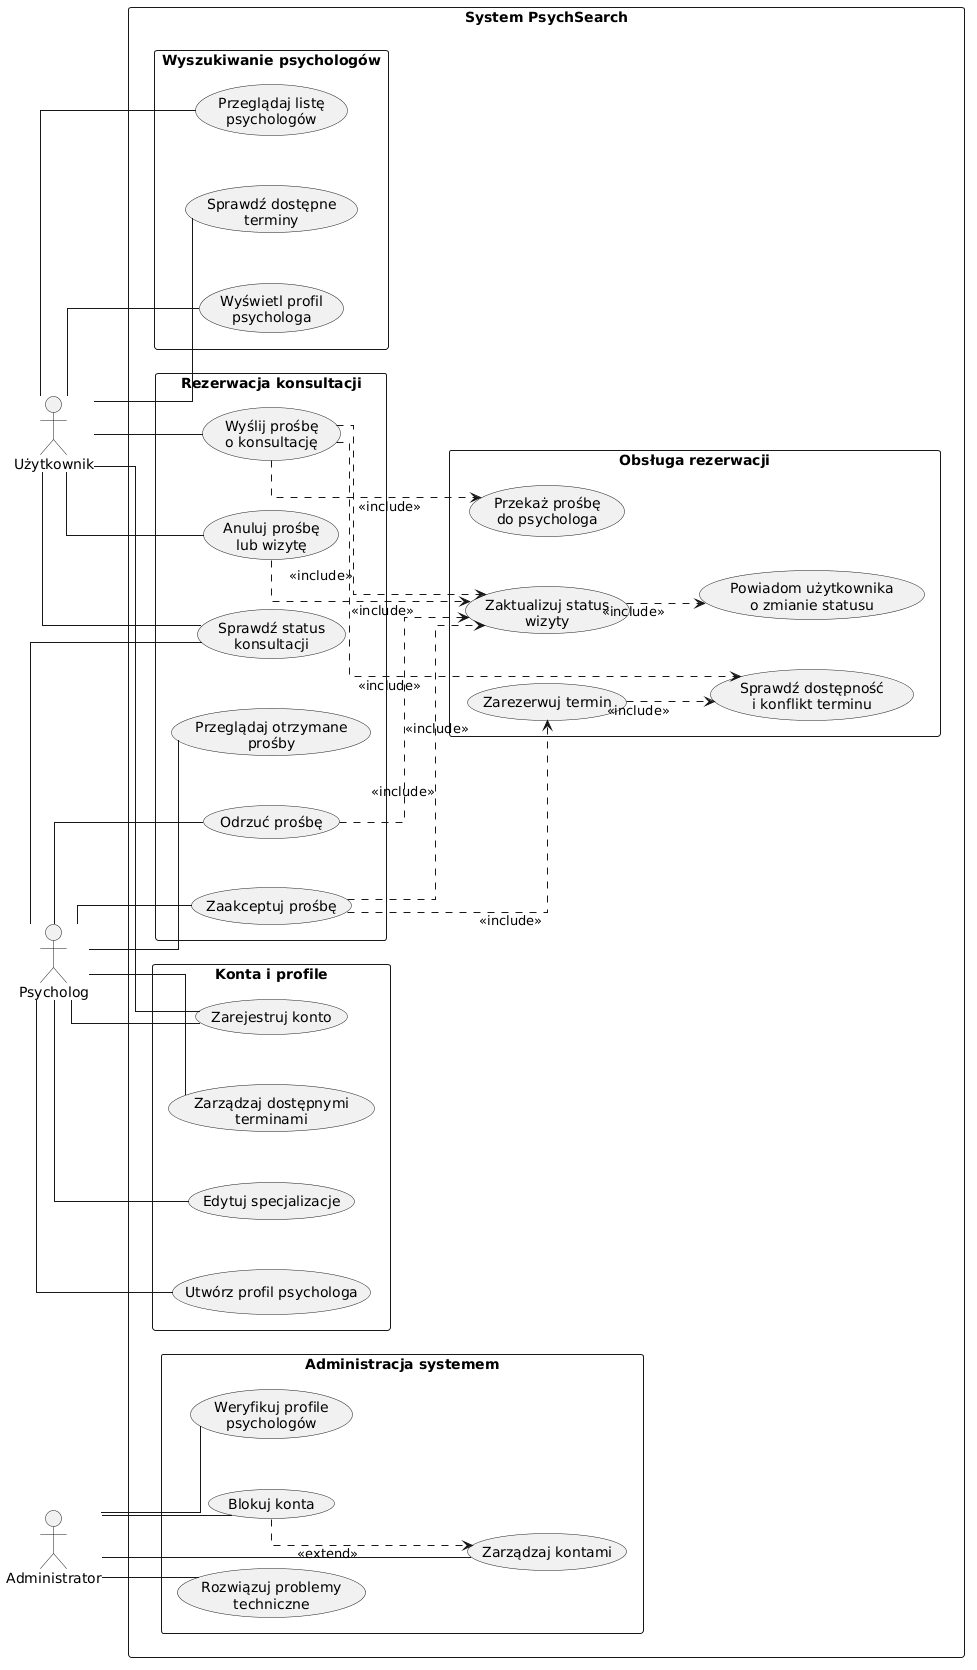
\includegraphics[width=\textwidth,height=0.7\textheight,keepaspectratio]{use_case_diagram.png}
    \label{fig:use_cases}
\end{figure}


\clearpage

\section*{Szczegółowe opisy funkcjonalności}

Opisy wybranych funkcjonalności systemu
według schematu opisu przypadku użycia.

\section*{Wysyłanie prośby o konsultację}

\begingroup
\small
\renewcommand{\arraystretch}{1.14}

\begin{tabularx}{\textwidth}{|p{3.9cm}|Y|}
\hline

\pole{Nazwa}{
Wysyłanie prośby o konsultację.
}

\pole{Krótki opis}{
Użytkownik prosi wybranego psychologa
o konsultację w określonym terminie.
}

\pole{Warunki początkowe}{
Użytkownik jest zalogowany, konto jest aktywne,
psycholog ma zweryfikowany profil
i udostępnione terminy.
}

\pole{Warunki końcowe}{
Prośba została zapisana ze statusem
„Oczekująca” i przekazana psychologowi.
Termin nie został jeszcze potwierdzony przez wybranego psychologa.
}

\pole{Sytuacje błędne}{
Termin nie jest dostępny albo nie udało się
zapisać prośby.
}

\pole{Stan po błędzie}{
Prośba nie powstaje, a użytkownik
otrzymuje komunikat.
}

\pole{Aktorzy}{
Użytkownik (główny),
psycholog (odbiorca prośby).
}

\pole{Wyzwalacz}{
Użytkownik wybiera opcję wysłania
prośby o konsultację.
}

\pole{Przebieg podstawowy}{
1. Użytkownik wybiera psychologa.\par
2. Przegląda wolne terminy i wybiera termin.\par
3. Potwierdza wysłanie prośby.\par
4. System sprawdza dostępność terminu.\par
5. System zapisuje prośbę jako „Oczekująca”.\par
6. System przekazuje prośbę psychologowi
i potwierdza wysłanie użytkownikowi.
}

\pole{Przebiegi alternatywne}{
3a. Użytkownik rezygnuje -
prośba nie zostaje zapisana.\par
4a. Termin jest niedostępny -
system umożliwia wybór innego.
}

\end{tabularx}
\endgroup

\clearpage

\section*{Akceptowanie prośby o konsultację}

\begingroup
\small
\renewcommand{\arraystretch}{1.14}

\begin{tabularx}{\textwidth}{|p{3.9cm}|Y|}
\hline

\pole{Nazwa}{
Akceptowanie prośby o konsultację.
}

\pole{Krótki opis}{
Psycholog zatwierdza prośbę,
potwierdzając możliwość odbycia konsultacji.
}

\pole{Warunki początkowe}{
Psycholog jest zalogowany,
a skierowana do niego prośba
ma status „Oczekująca”.
}

\pole{Warunki końcowe}{
Prośba ma status „Zaakceptowana”,
termin jest zarezerwowany,
użytkownik otrzymuje powiadomienie.
}

\pole{Sytuacje błędne}{
Prośba została anulowana albo zapis
rezerwacji się nie powiódł.
}

\pole{Stan po błędzie}{
Nie powstaje rezerwacja ani potwierdzenie
wizyty; psycholog widzi komunikat.
}

\pole{Aktorzy}{
Psycholog (główny),
użytkownik (odbiorca potwierdzenia).
}

\pole{Wyzwalacz}{
Psycholog wybiera opcję akceptacji prośby.
}

\pole{Przebieg podstawowy}{
1. Psycholog otwiera listę otrzymanych próśb.\par
2. Wybiera prośbę i sprawdza jej szczegóły.\par
3. Klika „Akceptuj”.\par
4. System ponownie weryfikuje status prośby
i dostępność terminu.\par
5. System zapisuje rezerwację
i nadaje jej status „Zaakceptowana”.\par
6. System powiadamia użytkownika.
}

\pole{Przebiegi alternatywne}{
3a. Psycholog nie zatwierdza prośby -
jej status pozostaje bez zmian.\par
4a. Termin jest już zajęty lub prośba
anulowana - akceptacja zostaje zablokowana.
}

\end{tabularx}
\endgroup

\clearpage

\section*{Anulowanie prośby lub wizyty}

\begingroup
\small
\renewcommand{\arraystretch}{1.14}

\begin{tabularx}{\textwidth}{|p{3.9cm}|Y|}
\hline

\pole{Nazwa}{
Anulowanie prośby lub wizyty.
}

\pole{Krótki opis}{
Użytkownik rezygnuje z oczekującej
prośby lub potwierdzonej konsultacji.
}

\pole{Warunki początkowe}{
Użytkownik jest zalogowany,
a wybrana konsultacja należy do niego
i ma status „Oczekująca” lub „Zaakceptowana”.
}

\pole{Warunki końcowe}{
Status zmienia się na „Anulowana”.
Jeśli termin był zarezerwowany,
zostaje zwolniony.
}

\pole{Sytuacje błędne}{
Próba wycofania konsultacji po przekroczeniu dozwolonego czasu na jej anulowanie lub wystąpienie błędu zapisu.
}

\pole{Stan po błędzie}{
Status i rezerwacja pozostają bez zmian;
użytkownik otrzymuje komunikat.
}

\pole{Aktorzy}{
Użytkownik.
}

\pole{Wyzwalacz}{
Użytkownik wybiera opcję
anulowania konsultacji.
}

\pole{Przebieg podstawowy}{
1. Użytkownik otwiera listę swoich konsultacji.\par
2. Wybiera prośbę lub wizytę.\par
3. Wybiera „Anuluj” i potwierdza decyzję.\par
4. System zmienia status na „Anulowana”.\par
5. System zwalnia termin,
jeśli był zarezerwowany.\par
6. System wyświetla potwierdzenie.
}

\pole{Przebiegi alternatywne}{
3a. Użytkownik rezygnuje -
status pozostaje bez zmian.\par
4a. Konsultacja nie może już być anulowana -
system odrzuca operację.
}

\end{tabularx}
\endgroup

\clearpage

\section*{Zarządzanie dostępnymi terminami}

\begingroup
\small
\renewcommand{\arraystretch}{1.14}

\begin{tabularx}{\textwidth}{|p{3.9cm}|Y|}
\hline

\pole{Nazwa}{
Zarządzanie dostępnymi terminami.
}

\pole{Krótki opis}{
Psycholog dodaje, edytuje i usuwa
wolne terminy w harmonogramie.
}

\pole{Warunki początkowe}{
Psycholog posiada profil w systemie i jest zalogowany.
}

\pole{Warunki końcowe}{
Harmonogram zawiera zapisane zmiany;
wolne terminy są widoczne dla użytkowników.
}

\pole{Sytuacje błędne}{
Konflikt z rezerwacją
lub próba usunięcia zajętego terminu.
}

\pole{Stan po błędzie}{
Zmiany nie zostają zapisane,
a psycholog otrzymuje komunikat.
}

\pole{Aktorzy}{
Psycholog.
}

\pole{Wyzwalacz}{
Psycholog otwiera zarządzanie harmonogramem.
}

\pole{Przebieg podstawowy}{
1. Psycholog otwiera harmonogram.\par
2. System wyświetla wolne i zajęte terminy.\par
3. Psycholog wybiera „Dodaj termin”.\par
4. Wybiera datę i godzinę.\par
5. System weryfikuje dane
i brak konfliktów.\par
6. Psycholog zatwierdza zmianę.\par
7. System zapisuje i wyświetla nowy termin.
}

\pole{Przebiegi alternatywne}{
3a. Psycholog edytuje istniejący wolny termin.\par
3b. Psycholog usuwa wolny termin.\par
5a. Termin koliduje z wizytą -
system odrzuca zmianę.
}

\end{tabularx}
\endgroup


\clearpage

\section*{Weryfikacja profili psychologów}

\begingroup
\small
\renewcommand{\arraystretch}{1.14}

\begin{tabularx}{\textwidth}{|p{3.9cm}|Y|}
\hline

\pole{Nazwa}{
Weryfikacja profili psychologów.
}

\pole{Krótki opis}{
Administrator sprawdza dane profilu
i decyduje o jego zatwierdzeniu
lub odrzuceniu.
}

\pole{Warunki początkowe}{
Administrator jest zalogowany, a profil oczekuje
na weryfikację.
}

\pole{Warunki końcowe}{
Profil otrzymuje status „Zweryfikowany”
albo „Odrzucony”; tylko profil
zweryfikowany jest udostępniany użytkownikom.
}

\pole{Sytuacje błędne}{
Brak wymaganych danych
lub problem podczas zapisu decyzji.
}

\pole{Stan po błędzie}{
Status profilu pozostaje bez zmian,
a profil nie zostaje opublikowany.
}

\pole{Przebieg podstawowy}{
1. Administrator otwiera listę
profili oczekujących.\par
2. Wybiera profil i analizuje podane dane.\par
3. Sprawdza wymagane kwalifikacje psychologa.\par
4. Zatwierdza profil.\par
5. System nadaje status „Zweryfikowany”.\par
6. Profil staje się widoczny dla użytkowników.
}

\pole{Przebiegi alternatywne}{
3a. Brakuje danych --
profil nadal oczekuje na weryfikację.\par
4a. Administrator odrzuca profil --
system zapisuje status „Odrzucony”
i nie publikuje profilu.
}

\end{tabularx}
\endgroup

\end{document}
